\chapter{Topic-Specific Guidelines}
\label{app:topic-specific_guidelines}

\section{IC design (ASIC or FPGA) projects}

    For \gls{ic} design projects, the part of the report where you present your main contributions (the \textsl{Implementation} chapter in this template) usually consists of two chapters: \textsl{Hardware Architecture} and \textsl{Design Implementation}.

  \subsection{Hardware architecture}

    In the Hardware Architecture chapter, you should describe the architecture and decisions that led to it.
    Block diagrams and descriptions of control flow, data flow, and interfaces go there.
    The described architecture can be more general than what you actually implemented, e.g., through parameters.

  \subsection{Design implementation}

    The Design Implementation chapter is about the architecture variant you actually implemented.
    It can be meaningful to merge this chapter with the Results chapter to relate central figures of merit directly to implementation choices and tradeoffs; discuss this with your advisors.

    \subsubsection{Functional verification}

      Describe how you verified the design implementation functionally.
      For example, describe how your testbench interfaced the golden model and your circuit.
      \Cref{fig:functional_verification_tb} illustrates a sample setup.

      \begin{figure}
        \centering
        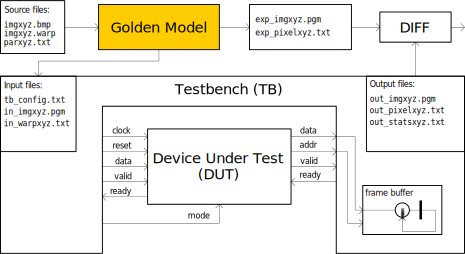
\includegraphics[width=\textwidth]{functional_verification_tb}
        \caption{Testbench used for functional verification.}%
        \label{fig:functional_verification_tb}
      \end{figure}

      Reference a ReadMe file that describes how the testbench can be launched.

    \subsubsection{Back-end implementation}

      In \gls{asic} projects, remember to discuss both front- and back-end implementation.
      That is, if you took special measures for floorplanning, \gls{dft}, or clock or power distribution, you will want to mention it here.
      In this case, make sure to add results that show the impact of your measures.

  \subsection{Results}

    Typical application-specific figures of merit of your hardware design are \gls{snr}, throughput, and memory/interface bandwidth.
    Moreover, you should also specify technology-specific figures such as area (for \glspl{asic}) or resource (for \glspl{fpga}) requirements, timing constraints, and power and energy consumption.

  \subsection{Data sheet}

    If your \gls{asic} is getting fabricated, you need to write a data sheet for it.
    You should put this data sheet into the appendix of your report.
    You are free to write the data sheet in a standalone document and include a \gls{pdf} file here or to write it in the source files of your report.

    Sections of a typical \gls{ic} data sheet are:
    \begin{itemize}
      \item Features
      \item Applications
      \item Packaging
      \item Bonding diagram like the one in \cref{fig:bonding_diagram}.
      \item Pinout diagram like the one in \cref{fig:asic_pinout}.
      \item Interface description
      \item Register map
      \item Operation modes:
      \begin{itemize}
        \item Functional modes
        \item Test modes
      \end{itemize}
      \item Electrical specifications
      \begin{itemize}
        \item Recommended operating regions
        \item Absolute maximum ratings
      \end{itemize}
    \end{itemize}

    \begin{figure}
      \centering
      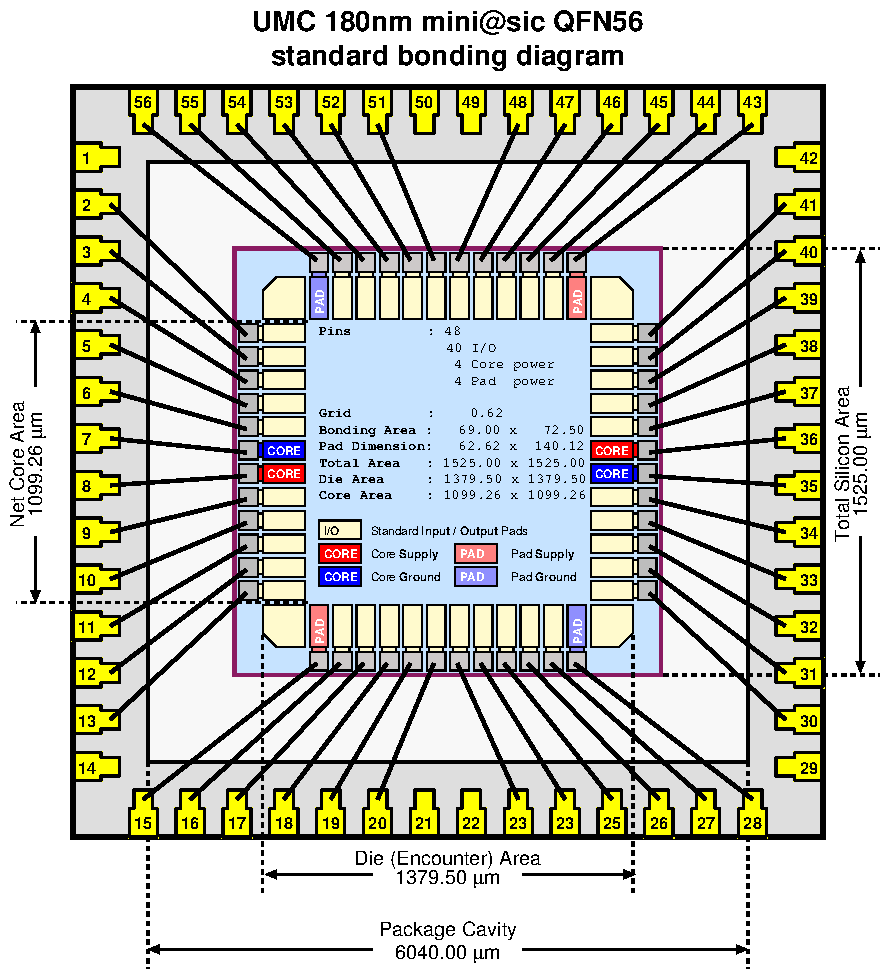
\includegraphics[width=.75\textwidth]{qfn56_180_std}
      \caption{Standard bonding diagram for QFN56 UMC 180\,nm mini@sics.}%
      \label{fig:bonding_diagram}
    \end{figure}

    \begin{figure}
      \centering
      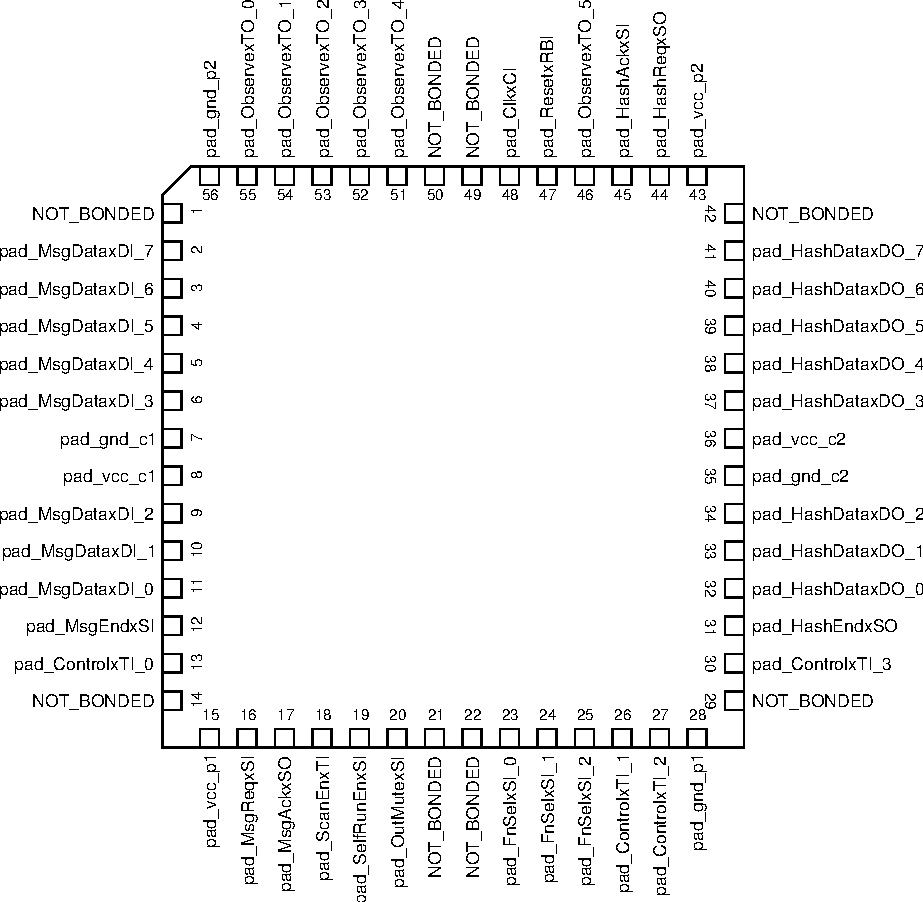
\includegraphics[width=.75\textwidth]{asic_pinout}
      \caption{Pinout for \textsc{MyFancyChip}.}%
      \label{fig:asic_pinout}
    \end{figure}

    For more information, up-to-date bonding diagrams, and other technology-specific data ask the \gls{dz}.
